\chapter{Calculation sample}

Author: Alvaro Ramirez

Descripcion del proceso: se tiene un proceso de aniquilacion directa de dos campos fermionicos(neutrinos derechos) a dos campos fermionicos(neutrinos izquierdos) $NN\to \nu\nu$.

\section{Lagrangiano}

Lagrangiano mas importante:

\begin {equation}
	\mathcal{L}_{Y}=f_{ij}({\phi}^{-}{\nu}_{i}+{\phi}^{0}{l}_{i}){l}_{i}^c+{h}_{ij}(\bar{{\nu}_{i}}{\eta}^0-{l}_{j}{\nu}^{\dagger}){N}_{j}+h.c
\end{equation}

Asi la parte relevante del lagrangino anterior es:

\begin {equation}
\mathcal{L}_{Y}={h}_{ij}(\bar{{\nu}_{i}}{\eta}^0-{l}_{j}{\nu}^{\dagger}){N}_{j}+hc
\end{equation}
\begin {equation}
\mathcal{L}_{Y}=h\bar{{\nu}_{3}}{\eta}^0{N}+h.c
\end{equation}
\begin {equation}
\mathcal{L}_{Y}=h\bar{{\nu}_{3}}{\eta}^0{N}+h(\nu_{3}{\eta}^{0}N)^{\dagger}
\end{equation}

\begin {equation}
\mathcal{L}_{Y}=h\bar{{\nu}_{3}}{\eta}^0{N}_{j}+h\bar{N}\eta^{0}\nu_{3}
\end{equation}


\section{S-matrix}

Calculo a segundo orden

\begin{gather}
\begin{split}
&<\nu(p'_{1})\nu(p'_{2})|(\bar{\nu}^{\alpha}_{+}(x_1)+\bar{\nu}^{\alpha}_{-}(x_1))({N}^{\alpha}_{+}(x_1)+\\&{N}^{\alpha}_{-}(x_1))(\bar{\nu}^{\beta}_{+}(x_2)+\bar{\nu}^{\beta}_{-}(x_2))(N^{\alpha}_{+}(x_2)+N^{\alpha}_{-}(x_2))|N(P_1)N(P_2)>\\
&=<\nu(p'_{1})\nu(p'_{2})|(\bar{\nu}^{\alpha}_{-}(x_1)({N}^{\alpha}_{+}(x_1)+{N}^{\alpha}_{-}(x_1)))(\bar{\nu}^{\beta}_{+}(x_2)+\\&\bar{\nu}^{\beta}_{-}(x_2)){N}^{\beta}_+(x_2)|N(P_1)N(P_2)>\\
&=<\nu(p'_{1})\nu(p'_{2})|\bar{\nu}^{\alpha}_{-}(x_1)({N}^{\alpha}_{+}(x_1)\bar{\nu}^{\beta}_{+}(x_2)+\\&{N}^{\alpha}_{+}(x_1)\bar{\nu}^{\beta}_{-}(x_2)+{N}^{\alpha}_{-}(x_1)\bar{\nu}^{\beta}_{+}(x_2)+{N}^{\alpha}_{-}(x_1)\bar{\nu}^{\beta}_{-}(x_2)){N}^{\beta}_{+}(x_2)|N(P_1)N(P_2)>\\
&=<\nu(p'_{1})\nu(p'_{2})|-\bar{\nu}^{\alpha}_{-}(x_1)(-\bar{\nu}^{\beta}_{+}(x_2){N}^{\alpha}_{+}(x_1)-\bar{\nu}^{\beta}_{-}(x_2){N}^{\alpha}_{+}(x_1)-\\&\bar{\nu}^{\beta}_{+}(x_2){N}^{\alpha}_{-}(x_1)-\bar{\nu}^{\beta}_{-}(x_2){N}^{\alpha}_{-}(x_1)){N}^{\beta}_{+}(x_2)|N(P_1)N(P_2)>\\
&=-<\nu(p'_{1})\nu(p'_{2})|\bar{\nu}^{\alpha}_{-}(x_1)\bar{\nu}^{\beta}_{-}(x_2){N}^{\alpha}_{+}(x_1){N}^{\beta}_{+}(x_2))|N(P_1)N(P_2)>\\
&=-\eta^{0}(x_1)\eta^{0}(x_2)<{\nu}^{\alpha}(p'_{1}){\nu}^{\beta}(p'_{2})|\bar{\nu}^{\alpha}_{-}(x_{1})\bar{\nu}^{\beta}_{-}(x_{2}){N}^{\alpha}_{+}(x_1){N}^{\beta}_{+}(x_2))|N(P_1)N(P_2)>\\
\end{split}
\end{gather}

\begin {equation}
|N(P_1)N(P_2)>=\frac{(2\pi)^{3}}{V}f^{\dagger}(p_2)f^{\dagger}(p_1)|0>
\end{equation}

\begin{gather}
\begin{split}
{N}^{\alpha}_{+}(x_1){N}^{\beta}(x_2)|N(\textbf{P}_1)N(\textbf{P}_2)>&= \int \frac{{d}^{3}k}{\sqrt{2E_{k}V}}\int \frac{{d}^{3}k'}{\sqrt{2E_{k'}V}}\nu^{\alpha}(k)\nu^{\beta}(k')e^{-ik-x_{1}}e^{-ik'-x_{2}}f(\textbf{k})\\&f(\textbf{k'})f^{\dagger}(\textbf{P}_2)f^{\dagger}(\textbf{P}_1)|0>
\end{split}
\end{gather}

haciendo uso de la siguiente identidad

\begin {equation}
[AB,CD]_{+}=A[B,C]_{+}D-[A,C]_{+}BD+CA[B,D]_{+}-C[A,D]_{+}B
\end {equation}

lo cual se cumple para cualesquier cuatro operadores A,B,C,D y utilizando las relaciones de anticonmutacion:

\begin {equation}
[f_s(\textbf{P}),f^{\dagger}_{s'}(\textbf{P'})]_{+}=[\hat{f}_{s}(\textbf{P}),\hat{f}^{\dagger}_{s'}(\textbf{P'})]_{+}=\delta_{ss'}\delta^{3}(\textbf{P}-\textbf{P'})
\end {equation}
se tiene

\begin{gather}
\begin{split}
[f(\textbf{K})f(\textbf{K'},f^{\dagger}(\textbf{P}_2)f^{\dagger}(\textbf{P}_1)]_+ &= f(\textbf{K})[f(\textbf{K'}),f^{\dagger}(\textbf{P}_2)]_+f^{\dagger}(\textbf{P}_1)-[f(\textbf{K}),f^{\dagger}(\textbf{P}_2)]_+f(\textbf{K'}f^{\dagger}(\textbf{P}_1)+\\&f^{\dagger}(\textbf{P}_2)f(\textbf{K})[f(\textbf{K'},f^{\dagger}(\textbf{P}_1)]_+-f^{\dagger}(\textbf{P}_2)[f(\textbf{K}),f^{\dagger}(\textbf{P}_1)]_+f(\textbf{K'})\\&=f(\textbf{K})\delta^{3}(\textbf{K'}-\textbf{P}_2)f^{\dagger}(\textbf{P}_1)-\delta^{3}(\textbf{K}-\textbf{P}_2)f(\textbf{K})f^{\dagger}(\textbf{P}_1)\\&+f^{\dagger}(\textbf{P}_2)f(\textbf{K})\delta^{3}(\textbf{K'}-\textbf{P}_1)-f^{\dagger}(\textbf{P}_2)\delta^{3}(\textbf{K}-\textbf{P}_1)f(\textbf{K'}
\end{split}
\end{gather}

\begin{gather}\begin{split}
[f(\textbf{K})f(\textbf{K'}),f^{\dagger}(\textbf{P}_2)f^{\dagger}(\textbf{P}_1)]_+&=\delta^{3}(\textbf{K'}-\textbf{P}_2)f(\textbf{K})f^{\dagger}(\textbf{P}_1)-\delta^{3}(\textbf{K}-\textbf{P}_2)f(\textbf{K'}f^{\dagger}(\textbf{P}_1)+\\&\delta^{3}(\textbf{K'}-\textbf{P}_1)f^{\dagger}(\textbf{P}_2)f(\textbf{K})-\delta^{3}(\textbf{K}-\textbf{P}_1)f^{\dagger}(\textbf{P}_2)f(\textbf{K'})
\end{split}
\end{gather}

Aplicando nuevamente las relaciones de anticonmutaciòn para $f(\textbf{P})$ y $f^{\dagger}(\textbf{P'})$ se tiene:

\begin{gather}
\begin{split}
[f(\textbf{K}),f^{\dagger}(\textbf{P}_1)]=\delta^{3}(\textbf{K}-\textbf{P}_1)\\
f(\textbf{K})f^{\dagger}(\textbf{P}_1)+f^{\dagger}(\textbf{P}_1)f(\textbf{K})=\delta^{3}(\textbf{K}-\textbf{P}_1)\\
f(\textbf{K})f^{\dagger}(\textbf{P}_1)=\delta^{3}(\textbf{K}-\textbf{P}_1)-f^{\dagger}(\textbf{P}_1)f(\textbf{K})\\
f(\textbf{K})f^{\dagger}(\textbf{P}_1)=\delta^{3}(\textbf{K}-\textbf{P}_1)
\end{split}
\end{gather}

ya que $f(\textbf{K})$ aniquila al vacio, analogamente para
\begin{gather}
\begin{split}
[f(\textbf{K'},f^{\dagger}(\textbf{P}_1)]=\delta^{3}(\textbf{K'}-\textbf{P}_1)\\
f(\textbf{K'}f^{\dagger}(\textbf{P}_1)+f^{\dagger}(\textbf{P}_1)f(\textbf{K'}=\delta^{3}(\textbf{K'}-\textbf{P}_1)\\
f(\textbf{K'}f^{\dagger}(\textbf{P}_1)=\delta^{3}(\textbf{K'}-\textbf{P}_1)-f^{\dagger}(\textbf{P}_1)f(\textbf{K'}
\end{split}
\end{gather}
ya que $f(\textbf{K'}$ aniquila al vacio

reemplazando los 2 resultados en (17)
\begin{gather}
\begin{split}
[f(\textbf{K})f(\textbf{K'},f^{\dagger}(\textbf{P}_2)f^{\dagger}(\textbf{P}_1)]=\delta^{3}(\textbf{K'}-\textbf{P}_2)\delta^{3}(\textbf{K}-\textbf{P}_1)-\delta^{3}(\textbf{K}-\textbf{P}_2)\delta^{3}(\textbf{K'}-\textbf{P}_1)
\end{split}
\end{gather}

por otro lado
\begin{gather}
\begin{split}
[f(\textbf{K})f(\textbf{K'}),f^{\dagger}(\textbf{P}_2)f^{\dagger}(\textbf{P}_1)]_{+}=f(\textbf{K})f(\textbf{K'})f^{\dagger}(\textbf{P}_2)f^{\dagger}(\textbf{P}_1)+f^{\dagger}(\textbf{P}_2)f^{\dagger}(\textbf{P}_1)f(\textbf{K})f(\textbf{K'})
\end{split}
\end{gather}

notese que el segundo termino del lado derecho aniquila el vacio luego,

\begin{gather}
\begin{split}
[f(\textbf{K})f(\textbf{K'}),f^{\dagger}(\textbf{P}_2)f^{\dagger}(\textbf{P}_1)]_{+}=f(\textbf{K})f(\textbf{K'})f^{\dagger}(\textbf{P}_2)f^{\dagger}(\textbf{P}_1)
\end{split}
\end{gather}

igualando 21 y 22

\begin{gather}
\begin{split}
f(\textbf{K})f(\textbf{K'})f^{\dagger}(\textbf{P}_2)f^{\dagger}(\textbf{P}_1)|0>=(\delta^{3}(\textbf{K'}-\textbf{P}_2)\delta^{3}(\textbf{K}-\textbf{P}_1)-\delta^{3}(\textbf{K}-\textbf{P}_2)\delta^{3}(\textbf{K'}-\textbf{P}_1))|0>
\end{split}
\end{gather}

reemplazando 8 en 13

\begin{gather}
\begin{split}
{N}^{\alpha}_{+}(x_1){N}^{\beta}_{+}(x_2)|{N}(\textbf{P}_1){N}(\textbf{P}_2)>&=\int \frac{{d}^{3}k}{\sqrt{2E_{k}V}}\int \frac{{d}^{3}k'}{\sqrt{2E_{k'}V}}\nu^{\alpha}(k)\nu^{\beta}(k')e^{-ik-x_{1}}e^{-ik'-x_{2}}\\&(\delta^{3}(\textbf{K'}-\textbf{P}_2)\delta^{3}(\textbf{K}-\textbf{P}_1)-\delta^{3}(\textbf{K}-\textbf{P}_2)\delta^{3}(\textbf{K'}-\textbf{P}_1))
\end{split}
\end{gather}

despues de integrar 

\begin{gather}
\begin{split}
{N}^{\alpha}_{+}(x_1){N}^{\beta}_{+}(x_2)|{N}(\textbf{P}_1){N}(\textbf{P}_2)>&=[\frac{1}{\sqrt{2E_{1}V}}\frac{1}{\sqrt{2E_{2}V}}\nu^{\alpha}({P}_1)\nu^{\beta}({P}_{2})e^{-i{P}_{1}-x_{1}}e^{-iP_{2}-x_{2}}-\\& \frac{1}{\sqrt{2E_{2}V}}\frac{1}{\sqrt{2E_{1}V}}\nu^{\alpha}({P}_2)\nu^{\beta}({P}_{1})e^{-i{P}_{2}-x_{1}}e^{-iP_{1}-x_{2}}])|0>
\end{split}
\end{gather}

en donde $E_{i}=\sqrt{\vec{P_i^2}+m^2}$ con $i=1,2$

\begin{gather}
\begin{split}
{N}^{\alpha}_{+}(x_1){N}^{\beta}_{+}(x_2)|{N}(\textbf{P}_1){N}(\textbf{P}_2)>&=\frac{1}{\sqrt{2E_{1}V}}\frac{1}{\sqrt{2E_{2}V}}[\nu^{\alpha}({P}_1)\nu^{\beta}({P}_2)e^{-i{P}_{1}-x_{1}}e^{-iP_{2}-x_{2}}-\\&\nu^{\alpha}({P}_2)\nu^{\beta}({P}_1)e^{-i{P}_{2}-x_{1}}e^{-iP_{1}-x_{2}}]|0>
\end{split}
\end{gather}

ahora se considerara el estado final

\begin{gather}
\begin{split}
<\nu({P'}_1)\nu({P'}_2)|\bar{\nu}^{\alpha}_{-}(x_1)nu(\textbf{P'}_2)>|\bar{\nu}^{\beta}_{-}(x_2)&=\frac{1}{\sqrt{2E'_{1}V}}\frac{1}{\sqrt{2E'_{2}V}}<0|[\bar{U}^{\alpha}(P'_1)\bar{U}^{\beta}(P'_2)]e^{i{P'}_{1}x_{1}}e^{i{P'}_{2}x_{2}}\\&-\bar{U}^{\alpha}(P'_2)\bar{U}^{\beta}(P'_1)]e^{i{P'}_{2}x_{1}}e^{i{P'}_{1}x_{2}}
\end{split}
\end{gather}

reemplazando (9) y (10) en ()

\begin{gather}
\begin{split}
\mathcal{S}^{2}_{fi}&=-\frac{(-ih)^2}{2!}\int{d^4x_1}\int{d^4x_2}\Delta_F(x_1-x_2)<\bar{\nu}(\textbf{P'}_1)\bar{\nu}(\textbf{P'}_2)|\bar{\nu}^\alpha_-(x_1)\bar{\nu}^\beta_-(x_2){N}^{\alpha}_{+}(x_1){N}^{\beta}_{+}(x_2)|N(P_1)N(P_2)>\\\mathcal{S}^{2}_{fi}&=-\frac{(-ih)^2}{2!}\int{d^4x_1}\int{d^4x_2}\int{\frac{d^4x_q}{{2\pi}^4}}i\Delta_{f}(q)e^{i{q}(x_{1}-x_{2})}[\bar{U}^{\alpha}(P'_1)\bar{U}^{\beta}(P'_2)]e^{i{P'}_{1}x_{1}}e^{i{P'}_{2}x_{2}}\\&-\bar{U}^{\alpha}(P'_2)\bar{U}^{\beta}(P'_1)]e^{i{P'}_{2}x_{1}}e^{i{P'}_{1}x_{2}}][\nu^{\alpha}({P}_1)\nu^{\beta}({P}_2)e^{-i{P}_{1}-x_{1}}e^{-iP_{2}-x_{2}}-\\&\nu^{\alpha}({P}_2)\nu^{\beta}({P}_1)e^{-i{P}_{2}-x_{1}}e^{-iP_{1}-x_{2}}][\frac{1}{\sqrt{2E_{1}V}}\frac{1}{\sqrt{2E_{2}V}}\frac{1}{\sqrt{2E'_{1}V}}\frac{1}{\sqrt{2E'_{2}V}}]
\end{split}
\end{gather}

La amplitud de Feynman a segundo orden en la expansion de la matriz S está dada por


\begin{gather}
\begin{split}
\mathcal{M}^{(2)}_{fi}&=(ih)^2[\bar{U}^{\alpha}({P'}_2)\bar{U}^{\beta}({P'}_1)i\Delta_f(P_1-P'_2)-\bar{U}^{\alpha}({P'}_1)\bar{U}^{\beta}({P'}_2)]i\Delta_f(P_1-P'_1)]{U}^{\alpha}({P}_1){U}^{\alpha}({P}_2)
\end{split}
\end{gather}

\begin{gather}
\begin{split}
{|\mathcal{M}_{fi}|}^2&=[\bar{U}^{\alpha}({P'}_2)\bar{U}^{\beta}({P'}1){U}^{\alpha}({P}_1){U}^{\beta}({P}_2)-\bar{U}^{\alpha}({P'}_1)\bar{U}^{\beta}({P'}_2){U}^{\alpha}({P}_1){U}^{\beta}({P}_2)][\bar{U}^{\alpha}({P'}_2)\bar{U}^{\beta}({P'}1)]{U}^{\alpha}({P}_1){U}^{\beta}({P}_2)-\\&\bar{U}^{\alpha}({P'}_1)\bar{U}^{\beta}({P'}_2){U}^{\alpha}({P}_1){U}^{\beta}({P}_2)]^\dagger
\end{split}
\end{gather}


permutando los centrales

\begin{gather}
\begin{split}
{|\mathcal{M}_{fi}|}^2&=[\bar{U}^{\alpha}({P'}_2){U}^{\alpha}({P}_1)\bar{U}^{\beta}({P'}_1){U}^{\beta}({P}_2)-\bar{U}^{\alpha}({P'}_1){U}^{\alpha}({P}_1)\bar{U}^{\beta}({P'}_2){U}^{\beta}({P}_2)][\bar{U}^{\alpha}({P'}_2){U}^{\alpha}({P}_1)\bar{U}^{\beta}({P'}_1){U}^{\beta}({P}_2)-\\&\bar{U}^{\alpha}({P'}_1){U}^{\alpha}({P}_1)\bar{U}^{\beta}({P'}_2){U}^{\beta}({P}_2]^\dagger
\end{split}
\end{gather}

haciendo el cambio de componentes a vectores

\begin{gather}
\begin{split}
{|\mathcal{M}_{fi}|}^2&=[\bar{U}({P'}_2){U}({P}_1)\bar{U}({P'}_1){U}({P}_2)-\bar{U}({P'}_1){U}({P}_1)\bar{U}({P'}_2){U}({P}_2)][\bar{U}({P'}_2){U}({P}_1)\bar{U}({P'}_1){U}({P}_2)-\\&\bar{U}({P'}_1){U}({P}_1)\bar{U}({P'}_2){U}({P}_2]^\dagger
\end{split}
\end{gather}

hallando el segundo termino del hermitico conjugado
\begin{gather}
\begin{split}
&[\bar{U}({P'}_2){U}({P}_1)\bar{U}({P'}_1){U}({P}_2)]^{\dagger}-[\bar{U}({P'}_1){U}({P}_1)\bar{U}({P'}_2){U}({P}_2)]^{\dagger}\\
&=[\bar{U}({P'}_1){U}({P}_2)]^{\dagger}[\bar{U}({P'}_2){U}({P}_1)]^{\dagger}-[\bar{U}({P'}_2){U}({P}_2)]^{\dagger}[\bar{U}({P'}_1){U}({P}_1)]^{\dagger}
\end{split}
\end{gather}

haciendo lo mismo para la anterior expresion

\begin{gather}
\begin{split}
=[\bar{U}({P}_2){U}({P'}_1)][\bar{U}({P}_1){U}({P'}_2)]-[\bar{U}({P}_2){U}({P'}_2)][\bar{U}({P}_1){U}({P'}_1)]
\end{split}
\end{gather}

ahora expresando en terminos de componentes

\begin{gather}
\begin{split}
&=[\bar{U}^{\alpha}({P}_2){U}^{\alpha}({P'}_1)\bar{U}^{\beta}({P}_1){U}^{\beta}({P'}_2)-\bar{U}^{\alpha}({P}_2){U}^{\alpha}({P'}_2)\bar{U}^{\beta}({P}_1){U}^{\beta}({P'}_1)]
\end{split}
\end{gather}


\begin{gather}
\begin{split}
{|\mathcal{M}_{fi}|}^2&=[\bar{U}^{\alpha}({P'}_2){U}^{\alpha}({P}_1)\bar{U}^{\beta}({P'}_1){U}^{\beta}({P}_2)-\bar{U}^{\alpha}({P'}_1){U}^{\alpha}({P}_1)\bar{U}^{\beta}({P'}_2){U}^{\beta}({P}_2)]\\&[\bar{U}^{\alpha}({P}_2){U}^{\alpha}({P'}_1)\bar{U}^{\beta}({P}_1){U}^{\beta}({P'}_2)-\bar{U}^{\alpha}({P}_2){U}^{\alpha}({P'}_2)\bar{U}^{\beta}({P}_1){U}^{\beta}({P'}_1)]
\end{split}
\end{gather}

\begin{gather}
\begin{split}
[{|\mathcal{M}_{fi}|}^2&=[\bar{U}^{\alpha}({P'}_2){U}^{\alpha}({P}_1)\bar{U}^{\beta}({P'}_1){U}^{\beta}({P}_2)][\bar{U}^{\alpha}({P}_2){U}^{\alpha}({P'}_1)\bar{U}^{\beta}({P}_1){U}^{\beta}({P'}_2)]-\\&[\bar{U}^{\alpha}({P'}_1){U}^{\alpha}({P}_1)\bar{U}^{\beta}({P'}_2){U}^{\beta}({P}_2)][\bar{U}^{\alpha}({P}_2){U}^{\alpha}({P'}_1)\bar{U}^{\beta}({P}_1){U}^{\beta}({P'}_2)]-\\&[\bar{U}^{\alpha}({P'}_2){U}^{\alpha}({P}_1)\bar{U}^{\beta}({P'}_1){U}^{\beta}({P}_2)][\bar{U}^{\alpha}({P}_2){U}^{\alpha}({P'}_2)\bar{U}^{\beta}({P}_1){U}^{\beta}({P'}_1)]+\\&[\bar{U}^{\alpha}({P'}_1){U}^{\alpha}({P}_1)\bar{U}^{\beta}({P'}_2){U}^{\beta}({P}_2)][\bar{U}^{\alpha}({P}_2){U}^{\alpha}({P'}_2)\bar{U}^{\beta}({P}_1){U}^{\beta}({P'}_1)]
\end{split}
\end{gather}

Efectuando la multiplicacion de los dos primero terminos
\begin{gather}
\begin{split}
&[\bar{U}^{\alpha}({P'}_2){U}^{\alpha}({P}_1)\bar{U}^{\beta}({P'}_1)\bar{U}^{\beta}({P}_1){U}^{\beta}({P}_2)][\bar{U}^{\alpha}({P}_2){U}^{\alpha}({P'}_1)\bar{U}^{\beta}({P}_1){U}^{\beta}({P'}_2)]\\&={U}^{\beta}({P'}_2)\bar{U}^{\alpha}({P'}_2){U}^{\alpha}({P}_1)\bar{U}^{\beta}({P}_1){U}^{\beta}({P}_2)\bar{U}^{\alpha}({P}_2)\bar{U}^{\beta}({P'}_1){U}^{\alpha}({P'}_1)
\end{split}
\end{gather}

\begin{gather}
\begin{split}
={U}^{\beta}({P'}_2)\bar{U}^{\alpha}({P'}_2){U}^{\alpha}({P}_1)\bar{U}^{\beta}({P}_1){U}^{\beta}({P}_2)\bar{U}^{\alpha}({P}_2){U}^{\alpha}({P'}_1)\bar{U}^{\beta}({P'}_1)
\end{split}
\end{gather}

\begin{gather}
\begin{split}
=&(P'_2+m'_2)_{\beta \alpha}(P'_1+m'_1)_{\alpha \beta}(P_2+m_2)_{\beta \alpha}(P_1+m_1)_{\alpha \beta}
\\&=Tr[(P'_2+m'_2)(P'_1+m'_1)]Tr[P_2+m_2)(P_1+m_1)]
\\&=Tr[(\gamma_{mu}P'_2{^\mu}+,m'_2)(\gamma_{nu}P'_1{^\nu}+,m'_1)]
\\&=4(P'_{2}.P'_{1}+m'_{1}m'{_2})
\end{split}
\end{gather}

de la misma forma

\begin{gather}
\begin{split}
&Tr[(P_2+m_2)(P_1+m_1)]Tr[P_2+m_2)(P_1+m_1)]
\\&=4(P_{2}.P_{1}+m_{1}m{_2})
\end{split}
\end{gather}

\begin{gather}
\begin{split}
{|\mathcal{M}_{fi}|}^2&=4({P'}_{2}.{P'}_{1}+{m'}_{1}{m'}_{2}).4(P_{2}.P_{1}+{m}_{1}m{_2}).4({P'}_{2}.{P'}_{1}+{m'}_{1}{m'}_{2}).4(P_{2}.P_{1}+m_{1}m{_2}).\\&4(P'_{2}.P'_{1}+m'_{1}m'{_2}).4(P_{2}.P_{1}+m_{1}m{_2}).4(P'_{2}.P'_{1}+m'_{1}m'{_2}).4(P_{2}.P_{1}+m_{1}m{_2})\\
{|\mathcal{M}_{fi}|}^2&=65536({P'}_{2}.{P'}_{1}+{m'}_{1}{m'}_{2})^{4}(P_{2}.P_{1}+{m}_{1}{m}_{2})^{4}
\end{split}
\end{gather}

tenemos que en CM
\begin{gather}
\begin{split}
\textbf{P}_1+\textbf{P}_2-\textbf{P'}_1+\textbf{P'}_2=0
\end{split}
\end{gather}

lo cual implica que
\begin{gather}
\begin{split}
&\textbf{P}_1=-\textbf{P}_2\\
&\textbf{P'}_1=-\textbf{P'}_2
\end{split}
\end{gather}

tomando en cuenta que $|\textbf{P'}_1|=\sqrt{{E'}_{1}^2-{m'}_{1}^2}$ se tiene

\begin{gather}
\begin{split}
&\textbf{P'}_1^2=\textbf{P'}_2^2\\
&{E'}_{1}^2-{m'}_{1}^2={E'}_{2}^2-{m'}_{2}^2\\
&{E'}_{2}^2={E'}_{1}^2-{m'}_{1}^2+{m'}_{2}^2
\end{split}
\end{gather}

Ademas, podemos definir la energia del centro de masa como
\begin{gather}
\begin{split}
\sqrt{s}=E_{1}+E_{2}
\end{split}
\end{gather}

igualmente se tiene
\begin{gather}
\begin{split}
|{P'}_{1}|=\sqrt{{E'}_{1}^{2}-{m'}_{1}^2}
\end{split}
\end{gather}

por otra parte
\begin{gather}
\begin{split}
{P}_{1}.{P}_{2}-{m}_{f}^{2}&={E}_{1}{E}_{2}-\textbf{P}_{1}.\textbf{P}_{2}-{m}_{1}{m}_{2}\\
&\frac{1}{2}[S^{2}-(m_{1}-m_{2})^{2}]
\end{split}
\end{gather}

\begin{gather}
\begin{split}
{P'}_{1}.{P'}_{2}=-{E'}_{1}{m}_{1}^{2}+{E'}_{1}{m}_{2}^{2}+2{E'}_{1}{m}_{1}-{m}_{1}^2
\end{split}
\end{gather}

considerando los siguientes dados iniciales 
\begin{gather}
\begin{split}
&{m}_{1}={m}_{2}=50 GeV\\
&{m'}_{1}={m'}_{2}=0 GeV\\
&{E}_{1}={E}_{2}=500 Gev\\
&{E'}_{1}={E'}_{2}=500 Gev\\
&{s}=10^{6}{GeV}^{2}
\end{split}
\end{gather}

\section{Process calculation}

Usando la ecuacion

\begin{equation}
  \frac{d\sigma}{d\Omega} = \frac{1}{64 \pi^2 s} \left\{ \frac{ [s-(m'_1 +m'_2)^2]}{[s-(m_1 + m_2)^2]} \frac{[s-(m'_1 - m'_2)^2 ]}{[s-(m_1 -m_2)^2]} \right\}^{\frac{1}{2}} | \bar{\mathcal{M}} |^2
\end{equation}


\begin{gather}
\begin{split}
\sigma=\frac{1}{64\pi^2s}{(\frac{s}{s-2m_{1}})}^{2}{|\mathcal{M}_{fi}|}^{2}\int{sen(\theta)}d\theta d\phi
\end{split}
\end{gather}


Reemplazando los valores predeterminados de (50) en (52), se tiene

\begin{gather}
\begin{split}
\sigma=10,110\times10^{-45}{cm}^{2}
\end{split}
\end{gather}

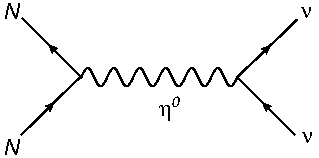
\includegraphics{imagen_1.pdf}

\section{CalcHEP comparison}

Check the result with CalcHEP. Please give the LanHEP code if necessaáry.

\section{Copyright}

\includegraphics[scale=0.5]{cc} Creative Commons Attribution-Share Alike 3.0 United States License.

%%% Local Variables:
%%% mode: latex
%%% TeX-master: "qft_samples"
%%% End:

